\subsection{Математическое ожидание и дисперсия}

    На графике \ref{EV_cyclic} для системы (\(\ref{beta_chaos}\)) (с \(\beta\)-шумом) представлены зависимости математического ожидания и дисперсии от параметра \(\beta\) и интенсивности шума \(\varepsilon\). На графике зависимости математического ожидания хорошо видно уменьшение параметрического интервала выживаемости популяции при увеличении интенсивности шума. Далее данное явление будет описано с помощью функции стохастической чувствительности.

    \begin{figure}
        \centering
        \subfloat[Математическое ожидание состояний системы]{
            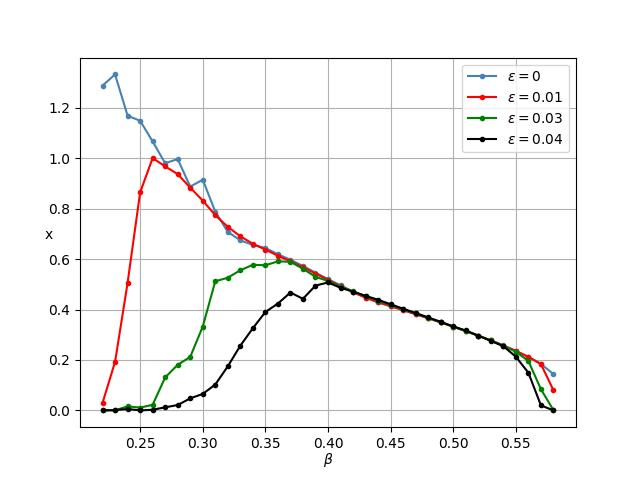
\includegraphics[width=0.5\textwidth]{stochastic/images/EV_cyclic.jpg}
            \label{EV_cyclic}
        }  
        \subfloat[Дисперсия состояний системы]{
            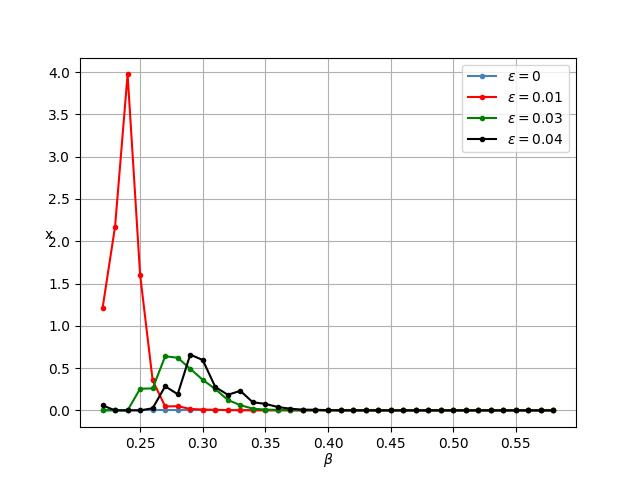
\includegraphics[width=0.5\textwidth]{stochastic/images/variance_cyclic.jpg}
            \label{variance_cyclic}
        }
        
        \caption{Бифуркационная диаграмма модели (\ref{beta_chaos}) (с \(\beta\)-шумом), \(\varepsilon = 0.01\)}
    \end{figure}
        
    % \begin{figure}
    %     \centering
    %     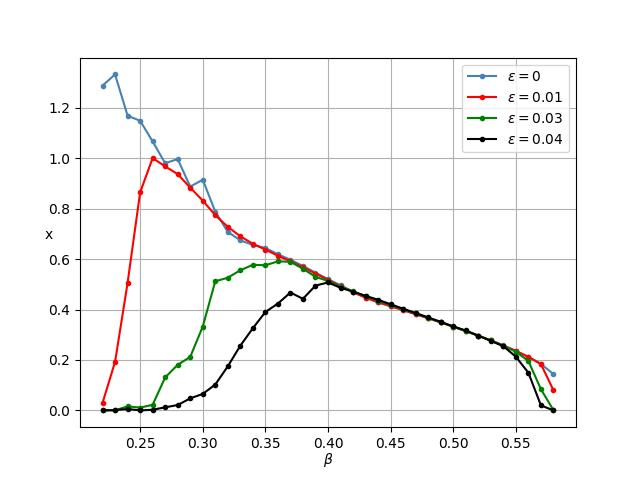
\includegraphics[width=0.5\textwidth]{stochastic/images/EV_cyclic.jpg}
        
    %     \captionsetup{justification=centering}
    %     \caption{Математическое ожидание состояний системы \(\ref{beta_chaos}\) (для \(\beta\)-шума)}
    %     \label{EV_cyclic}
    % \end{figure}

    % \begin{figure}
    %     \centering
    %     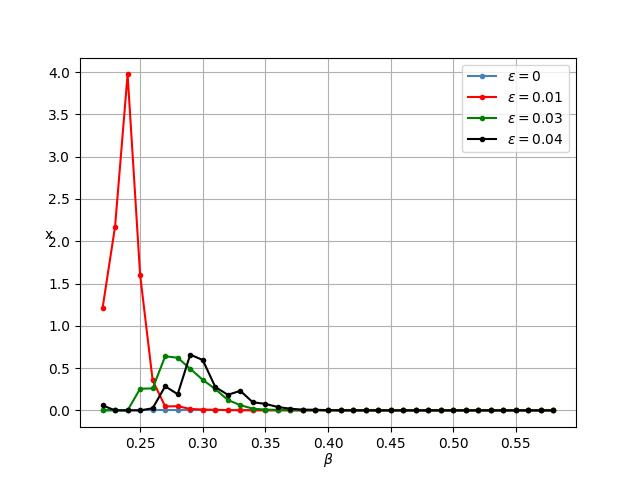
\includegraphics[width=\textwidth]{stochastic/images/variance_cyclic.jpg}
        
    %     \captionsetup{justification=centering}
    %     \caption{Дисперсия состояний системы (\ref{beta_chaos}) (для \(\ref{beta_chaos}\))}
    %     \label{variance_cyclic}
    % \end{figure}
